% file: decision-tree-selection-sort.tex

\documentclass{standalone}
\usepackage{tikz}
\usepackage{tikz-qtree}
\usetikzlibrary{shapes}

\begin{document}
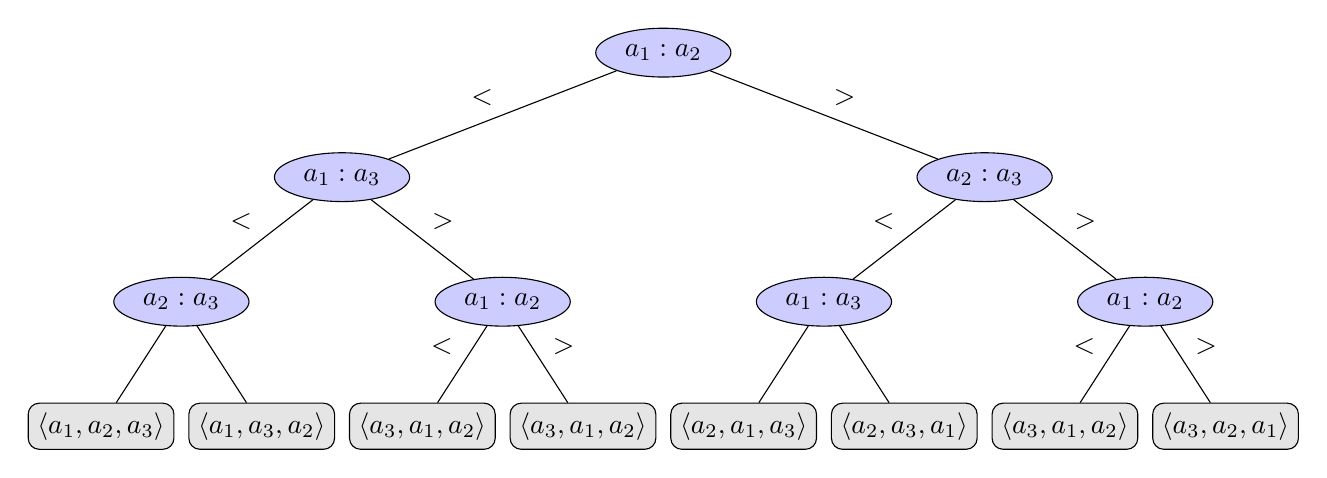
\begin{tikzpicture}[level distance = 45pt, sibling distance = 5pt,
  edge from parent/.style= { % added code
      draw, edge from parent path = {(\tikzparentnode) -- (\tikzchildnode)}},
    leaf/.style = {rectangle, rounded corners, fill = lightgray!40}]
  \tikzset{every tree node/.style = 
    {align = center, ellipse, draw, fill = blue!20}}

    \Tree [.{$a_1 : a_2$}	
	\edge node[auto = right]{$<$}; [.{$a_1 : a_3$} 
	    \edge node[auto = right]{$<$}; [.{$a_2 : a_3$}
	      [.\node[leaf]{$\langle a_1, a_2, a_3 \rangle$}; ]
	      [.\node[leaf]{$\langle a_1, a_3, a_2 \rangle$}; ]
	    ] 
	    \edge node[auto = left]{$>$};    [.{$a_1 : a_2$} 
	      	\edge node[auto = right]{$<$}; [.\node[leaf]{$\langle a_3, a_1, a_2 \rangle$}; ]
		\edge node[auto = left]{$>$};    [.\node[leaf]{$\langle a_3, a_1, a_2 \rangle$}; ]
		  ]
                ]
	\edge node[auto = left]{$>$}; [.{$a_2 : a_3$} 
	    \edge node[auto = right]{$<$}; [.{$a_1: a_3$}
	      [.\node[leaf]{$\langle a_2, a_1, a_3 \rangle$}; ]
	      [.\node[leaf]{$\langle a_2, a_3, a_1 \rangle$}; ]
	    ] 
	    \edge node[auto = left]{$>$}; [.{$a_1 : a_2$} 
		\edge node[auto = right]{$<$}; [.\node[leaf]{$\langle a_3, a_1, a_2 \rangle$}; ] 
		\edge node[auto = left]{$>$};	 [.\node[leaf]{$\langle a_3, a_2, a_1 \rangle$}; ] 
		  ]
		] 
	  ]
  \end{tikzpicture}
\end{document}
